\section{Evaluating Descriptors and Trajectories}
\label{sec:experiments}

Because no previous work explores the interpretability of
unsupervised relationship modeling over time, evaluating the \rmn\ is
tricky. Further compounding the problem is the subjective nature of
the task; for example, is a trajectory that ignores a key event better
than one that hallucinates episodes absent from source text?

With these issues in mind, we conduct three evaluations to show that our output
is reasonable. First, we conduct a crowdsourced interpretability experiment that
shows \rmn s produce significantly more coherent descriptors than three topic
model baselines. A second crowdsourced task indicates that our model produces
trajectories that match plot summaries more accurately than topic
models. Finally, we qualitatively compare the \rmn's output to existing static
annotations of literary relationships and find both expected and surprising
results.

\subsection{Topic Model Baselines}

Before moving onto the evaluations, we briefly describe three baseline models,
all of which are Bayesian generative models. Latent Dirichlet
allocation~\cite[\lda{}]{blei2003latent} learns a single document-topic
distribution per document; we can apply \lda\ to our dataset by concatenating
all spans from a relationship into a single document. Similarly,
\nubbi~\cite{chang2009connections} learns separate sets of topics for
relationships and individual characters.\footnote{\nubbi\ requires additional
  spans that mention only a single character to differentiate character topics
  from relationship topics. None of the other models receives these extra data.}

\lda\ and \nubbi\ are incapable of taking into account the chronological
ordering of the spans because they view all relationships tokens as
exchangeable. While we can compare the \emph{descriptors} learned by these
models to those of the \rmn, we cannot evaluate their \emph{trajectories}. We
turn instead to the hidden topic Markov model~\cite[\htmm]{gruber2007hidden},
which foregoes the bag-of-words assumption of \lda\ and \nubbi\ in favor of
modeling topic segments within a document as a Markov chain. This model outputs
a smooth sequence of topic assignments over a document, so we can compare the
\emph{trajectories} it learns on our dataset to those of the \rmn.

\subsection{Experimental Settings}

In our descriptor interpretability experiments, we vary the number of
descriptors (topics) for all models ($K=10,30,50$). We train \lda\ and
\nubbi\ for 100 iterations with a collapsed Gibbs sampler, and the \htmm\ uses
the default setting of 100 \abr{em} iterations.










For the \rmn, we initialize the word embedding matrix \bmat{L} with
300-dimensional GloVe embeddings trained on the Common
Crawl~\cite{glove2014}. The character and book embeddings (\bmat{C} and
\bmat{B}) are initialized randomly. We fix $\alpha$ to 0.5 for the first 15
epochs of training; after the descriptor matrix \bmat{R}\ has converged, we fix
\bmat{R}\ and tune $\alpha$ using Equation~\ref{eq:rmn} for 15 more
epochs.\footnote{Preliminary experiments show that learning $\alpha$ and
  \bmat{R} simultaneously results in less interpretable descriptors.} Since the
topic model baselines do not have access to character and book metadata, for
fair comparison we also train a ``generic'' version of the \rmn\ (\grmn) where
the metadata embeddings are removed from Equation~\ref{eq:dan}. The uniqueness
penalty $\lambda$ is set to $10^{-4}$.








All of the \rmn\ model parameters except \bmat{L} are optimized using
Adam~\cite{kingma2014adam} with a learning rate of 0.001 for 30 epochs; the word
embeddings are not fine-tuned during training.\footnote{Tuning \bmat{L} ruins
  descriptor interpretability; pretrained embeddings are likely already a good
  solution for our problem.} We also apply word dropout~\cite{IyyerDAN} to the
input spans, removing words from the vector average computation in
Equation~\ref{eq:ave} with probability 0.5.

\begin{table*}[ht]
\centering
\begin{tabular}{llp{5cm}llp{5cm}}
\toprule
\multicolumn{3}{c}{\bf RMN} & \multicolumn{3}{c}{\bf HTMM} \\
\cmidrule(l{10pt}r{10pt}){1-3}
\cmidrule(l{10pt}r{10pt}){4-6}
\bf Label & \bf MP & \bf Nearest Neighbors & \bf Label & \bf MP & \bf Most Probable Words \\
\midrule
sadness & 1.0 & \footnotesize regretful rueful pity pained despondent & violence & 1.0 & \footnotesize sword shot blood shouted swung \\
love & 1.0 & \footnotesize love delightful happiness enjoyed & boats & 1.0 & \footnotesize ship boat captain deck crew \\
murder & 1.0 & \footnotesize autopsy arrested homicide murdered & food & 1.0 & \footnotesize kitchen mouth glass food bread \\
\midrule
worship & 0.1 & \footnotesize toil pray devote yourselves gather & sci-fi & 0.0 & \footnotesize suppose earth robots computer certain \\
moodiness & 0.3 & \footnotesize glumly snickered quizzically guiltily & fantasy & 0.0 & \footnotesize agreed magician dragon castle talent\\
informal & 0.4 & \footnotesize kinda damn heck guess shitty& military & 0.1 & \footnotesize ship captain lucky hour general \\
\bottomrule
\end{tabular}

\caption{Three high-precision (top) and three low-precision (bottom) descriptors for the \rmn\ and \htmm, along with labels from an external evaluator and model precision (\abr{mp}) computed via word intrusion experiments. The \rmn\ is able to learn a variety of interpersonal states (e.g., \underline{love}, \underline{sadness}), while the \htmm's most coherent topics are about concrete objects or events.}
\label{table:intrusion}
\end{table*}

\subsection{Do Descriptors Make Sense?}

\begin{figure}[t!]
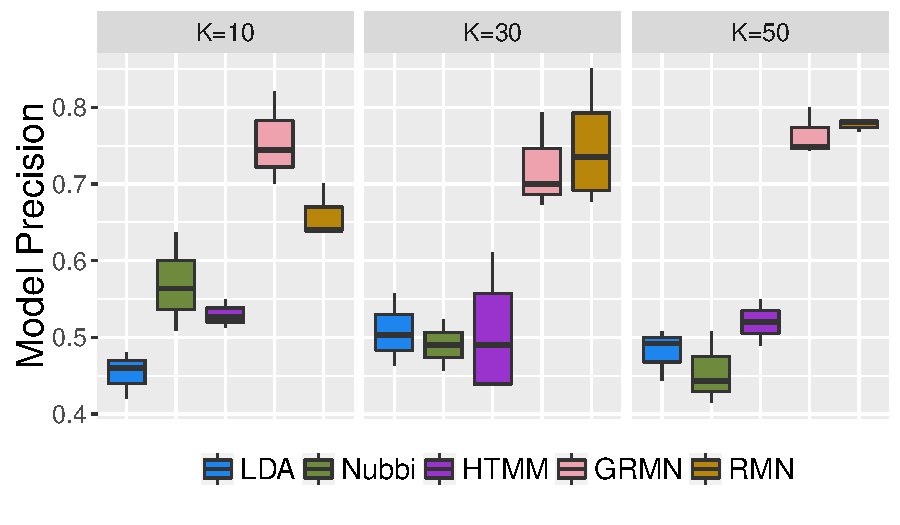
\includegraphics[width=1.0\linewidth]{2016_naacl_relationships/figures/topic_intrusion.pdf}
  \caption{Model precision results from our word intrusion task. The \rmn\
  learns more interpretable descriptors than three topic model baselines.}
\label{fig:intrusion}
\end{figure}

The goal of our first experiment is to compare the descriptors
\bmat{R} learned by the \rmn\ to the topics learned by the topic model
baselines. We conduct a word intrusion
experiment~\cite{chang2009reading}: workers identify an ``intruder''
word from a set of words that---other than the intruder---come from
the same topic. For the topic models, the five most probable words are
joined by a highly-probable word from a different topic as the
intruder. We use the same procedure for the \rmn\ and \grmn, except that
cosine similarity to descriptor embeddings replaces topic-word
probability. To control for randomness in the training process, we
train three of each model, so the final experiment consists of 1,350
tasks ($K=10,30,50$ descriptors per trial, three trials per model).

We collect judgments from ten different workers for each task using the
Crowdflower platform.\footnote{\url{http://www.crowdflower.com}} Our evaluation
metric, model precision (\abr{mp}), is the fraction of workers that select the
correct intruder word for a descriptor $k$.  Low model precision signals
descriptors that lack cohesive themes.

On average, the \rmn's descriptors are much more interpretable than those of the
baselines, as it achieves a mean model precision of 0.73
(Figure~\ref{fig:intrusion}) across all values of $K$.  There is little
difference between the model precision of the three topic model baselines,
which hover around 0.5. There is also little difference between the \grmn\ and
\rmn; however, visualizing the learned character and book embeddings as in
Figure~\ref{fig:bookpca} may be insightful for literary scholars. We show
example high and low precision descriptors for the \rmn\ and \htmm\ in
Table~\ref{table:intrusion}; a full list is included in the supplementary
material.

\subsection{Do Trajectories Make Sense?}

While the previous evaluation focused only on descriptor quality, our next
experiment compares the trajectories learned by the best \rmn\ model from the
intrusion experiment (measured by highest mean model precision) to those learned
by the best \htmm\ model, which is the only baseline capable of learning
relationship trajectories. Workers read a plot summary and choose which model's
trajectory best represents the relationship in question. We use the $K=30$
setting because it provides the best balance between descriptor variety and
trajectory interpretability.

For this evaluation, we crawl Wikipedia, Goodreads, and SparkNotes for plot
summaries associated with our 1,383 books. We then remove all relationships
where each involved character is not mentioned at least five times in the
summary, which results in a final evaluation set of 125
relationships.\footnote{Without this filtering step, workers do not have enough
  information to compare the two models since most of the characters in our
  dataset are not mentioned in summaries.}  We present workers with two
characters, a plot summary, and a visualization of trajectories learned by the
\rmn\ and the \htmm\ (Figure~\ref{fig:cftask}). The workers then select the
trajectory that best matches the relationship described by the summary.

To generate the visualizations, we first have an external annotator label each
descriptor from both models with a single word as in
Table~\ref{table:intrusion}. For fairness, the annotator is unaware of the
underlying models. For the \rmn, we visualize trajectories by displaying the
label of the argmax over descriptor weights $\bvec{d}_t$ at each time step
$t$. Similarly, for the \htmm, we display the most probable topic at each time
step.\footnote{To reduce visual clutter, we ignore descriptors that persist for
  only a single time step.}

The results of this task with seven workers per comparison favor the \rmn: for
87 out of the 125 evaluated relationships (69.6\%), the workers choose the
\rmn's trajectory over the \htmm's. We compute the Fleiss $\kappa$
value~\cite{fleiss1971measuring} to correct our inter-annotator agreement for
chance and find that $\kappa = 0.32$, indicating fair agreement among the
workers. Furthermore, thirty-four relationships had unanimous agreement among the seven
workers; of these, twenty-six were unanimous in favor of the \rmn\ compared to only eight
for the \htmm.

\begin{figure}[t!]
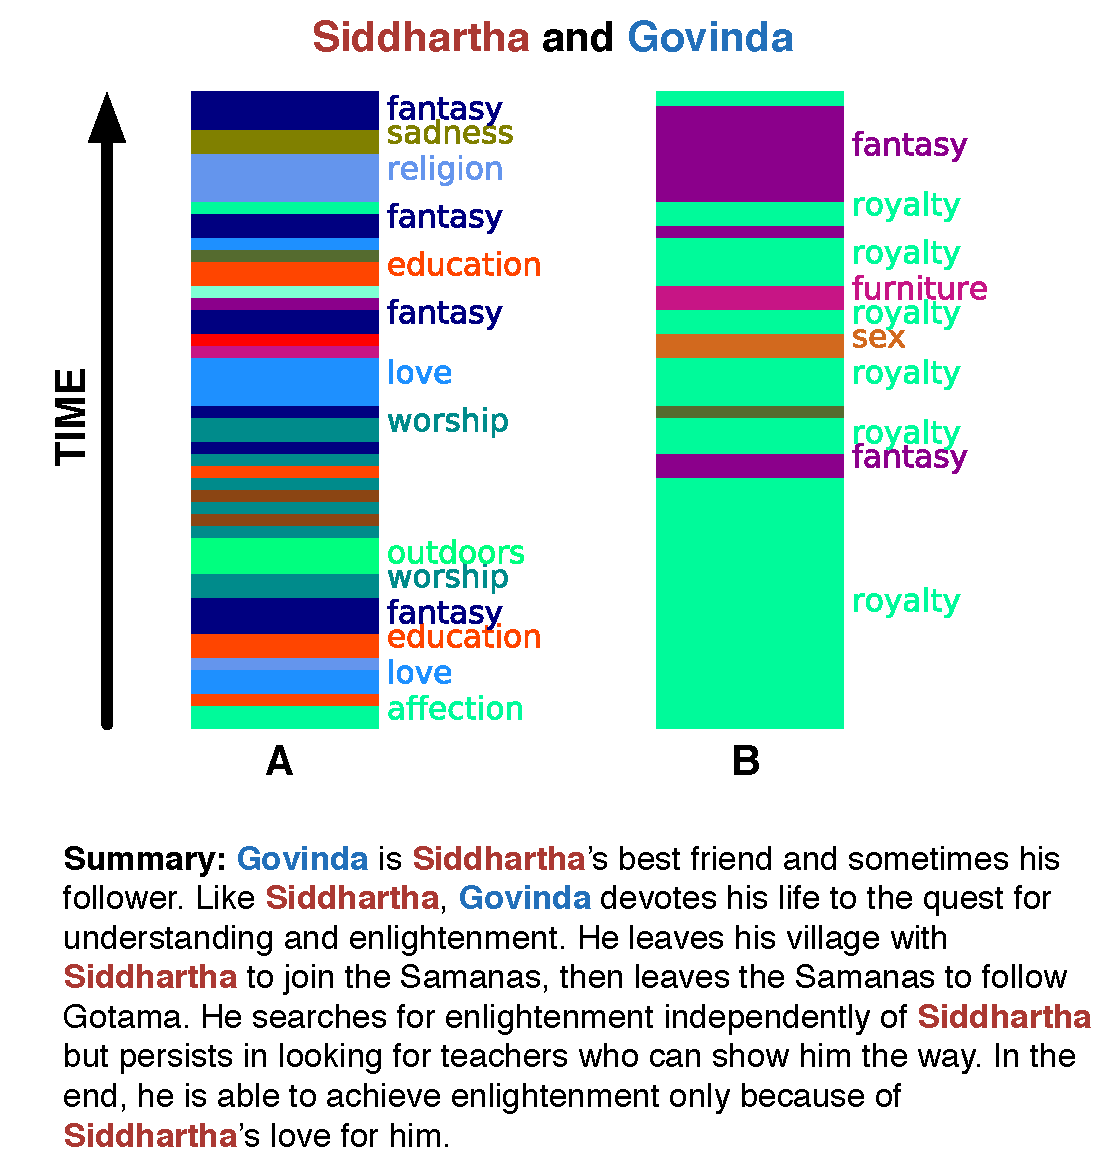
\includegraphics[width=1.0\linewidth]{2016_naacl_relationships/figures/cftask.pdf}
  \caption{An example from the Crowdflower summary matching task;
    workers are asked to choose the trajectory (here, ``A'' is generated by the
    \rmn\ and ``B'' by the \htmm) that best matches a provided summary that
    describes the relationship between Siddartha and Govinda (from
    \textit{Siddartha} by Hesse).}
\label{fig:cftask}
\end{figure}

\subsection{What Makes a Relationship Positive?}

While the previous two experiments show that the \rmn\ is more interpretable and
accurate than baseline models, we have not yet shown that its insights can aid
in drawing connections across various books and genres. As a first step in this
direction, we investigate what makes a relationship positive or negative by
comparing trajectories from the \rmn\ and \htmm\ to static affinity annotations
from a recently-released dataset~\cite{massey2015annotating} of fictional
relationships. Expected correlations (e.g., \underline{murder} and
\underline{sadness} are strongly negative descriptors) emerge alongside
surprising ones (\underline{politics} is negative, \underline{religion} is
positive).

The affinity labeling task of \newcite{massey2015annotating} requires workers to describe a given
relationship as positive, negative, or neutral. We consider only
non-neutral relationships for which two annotators agree on the affinity label and
remove all books not present in our own dataset. This filtering step results in 120
relationships, 78\% of which are positive and the remaining 22\% negative.

Since the annotations are static, we first aggregate our trajectories
across all time steps. We compute $K$-dimensional ``average positive'' and
``average negative'' weight vectors $\bvec{a}_p$ and $\bvec{a}_n$ by averaging
the relationship states $\bvec{d}_t$ for the \rmn\ and the document-topic
distributions for the \htmm\ across all time steps for relationships labeled
with a particular affinity. Then, we compute the vector difference $\bvec{a}_p -
\bvec{a}_n$ and sort it to produce a ranked list of descriptors, where
descriptors with positive differences occur more frequently in positive
relationships. Table~\ref{table:affinity} shows the most positive and most
negative descriptors; of particular interest is the large negative weight associated with political relationships from both models.

\begin{table}[t!]
\centering
\begin{tabular}{lp{2.8cm}p{2.8cm}}
\toprule
\bf Model & \bf Positive & \bf Negative\\
\midrule
\rmn & \footnotesize education, \textcolor{blue}{love}, religion, \textcolor{blue}{sex} & \footnotesize politics, \textcolor{red}{murder}, \textcolor{red}{sadness}, royalty \\
\htmm & \footnotesize \textcolor{blue}{love}, \textcolor{blue}{parental}, business, outdoors & \footnotesize \textcolor{blue}{love}, politics, \textcolor{red}{violence}, \textcolor{red}{crime} \\
\bottomrule
\end{tabular}

\caption{Descriptors most characteristic of positive and negative relationships,
  computed using existing annotations. Compared to the \rmn, the
  \htmm\ struggles to coherently characterize negative relationships. Interestingly, both models show negative predispositions for political
  relationships, perhaps due to genre bias or class differences. }

\label{table:affinity}
\end{table}
